\chapter{Eliminación de palabras}

En los capítulos anteriores, el relacionar las palabras migrantes con campos semánticos y eventos históricos que justifiquen su aparición, permitió establecer un forma para cuantificar la influencia entre idiomas llamado uso. Todo este método se facilitó por la eliminación de las palabras funcionales, dejando sólo palabras de contenido, pero ¿cómo se modificaría el uso entre idiomas,  si se eliminaran otro tipo de palabras, sin importar si estás son de contenido?

Esta pregunta ha llevado a la construcción de un nuevo algoritmo para reducir el conjunto de las palabras migrantes y obtener nuevos valores del uso entre idiomas.  Elegidos una pareja de idioma origen \textit{A} e idioma receptor \textit{B}, el proceso es el siguiente. 


\begin{enumerate}
	
	\item Se toma la lista de los préstamos acumulados de \textit{A} en \textit{B},  este corpus se denotará como \textbf{conjunto original}.
	
	\item Se escogen de forma aleatoria un grupo de letras (desde una hasta diez), y se descartan del conjunto original a aquellas  palabras cuya primer letra sea alguna de las elegidas. El nuevo corpus se denotará como \textbf{conjunto reducido}.
	
	\item Se establece un corpus  designado como \textbf{conjunto residuo}, conformado por todas las palabras eliminadas del conjunto original.  La unión del reducido y el residuo es el original. 
	
	\item En los tres conjuntos se emplea la ecuación \ref{ec.fuso}, para encontrar el uso de \textit{A} en \textit{B}. 	
	
\end{enumerate}

La intención de estas eliminación  no es desaparecer el conjunto de las migraciones, sino el reducirlas para  comparar el uso entre el conjunto original y el reducido.  Para determinar que tanto ha cambiado el uso en los dos conjuntos, se utilizará el coeficiente de determinación $R^{2}$. 

El primer criterio importante sera al tomar el uso en el conjunto original como verdadero (ya que con el se establecieron los resultados del capítulo anterior),  donde sus valores para un tiempo $t$ se expresan como $O_{t}$. Si el uso en el conjunto reducido para el mismo $t$ se denotan como  $v_{t}$ y el promedio de ellos es $\bar{v}$, entonces  el coeficiente de determinación queda definido como:

\begin{equation}
\label{ec.dif_uso}
R^{2} = 1 - \sum_{t} \frac{ \left( v_{t}- O_{t} \right)^{2}  }{ \left( v_{t} - \bar{v} \right)^{2} }.
\end{equation}

Se empleará el concepto \textbf{conservación del uso} para aquellos idiomas cuyo uso no cambie a pesar de las omisiones. La conservación es favorable si $R^{2}$ es próximo a 1. 
%Si la conservación no es favorable, las palabras eliminadas son las más relevantes para las migraciones de \textit{A} en \textit{B}.

\section{Características de las eliminaciones}

El procedimiento para eliminar palabras, obteniendo el uso y el coeficiente de determinación, se realizó dos mil veces por cada pareja de idiomas.  Tras las repeticiones, se distinguieron las siguientes características al graficar el uso de los conjuntos original y reducido. 


\begin{itemize}
	
	\item Valores iguales. Punto a punto el conjunto reducido empalma al original, por lo que las graficas son indistinguibles. La conservación del uso se da en todo el intervalo de tiempo. 
	
	\item Diferencia de alturas. Ambas gráficas muestran el mismo comportamiento, sin embargo existe una diferencia casi constante entre
	los valores del uso de ambos conjuntos. En este caso el uso también se conserva, ya que ambas graficas son las mismas sólo que sus valores están desfasados. 
	
	\item Alteraciones por periodos.  Se presentan periodos donde el uso de ambos conjuntos son completamente diferentes. La conservación se da por periodos cortos de tiempo e incluso puede ser inexistente.
	
\end{itemize}

Para ilustrar las caracterizaras mencionadas, se exponen algunas graficas obtenidas, representado con un trazo continuo al uso del conjunto original, mientras que el uso en el conjunto reducido  es una serie de puntos.   Ya que los valores en el conjunto residuo son muy pequeños, se opto por no graficarlos, para no saturar la información. 

En cada grafica se especifican los idiomas que intervienen, así como el conjunto de letras con las cuales se hicieron las eliminaciones. 



\begin{figure}[h!]
	\centering
	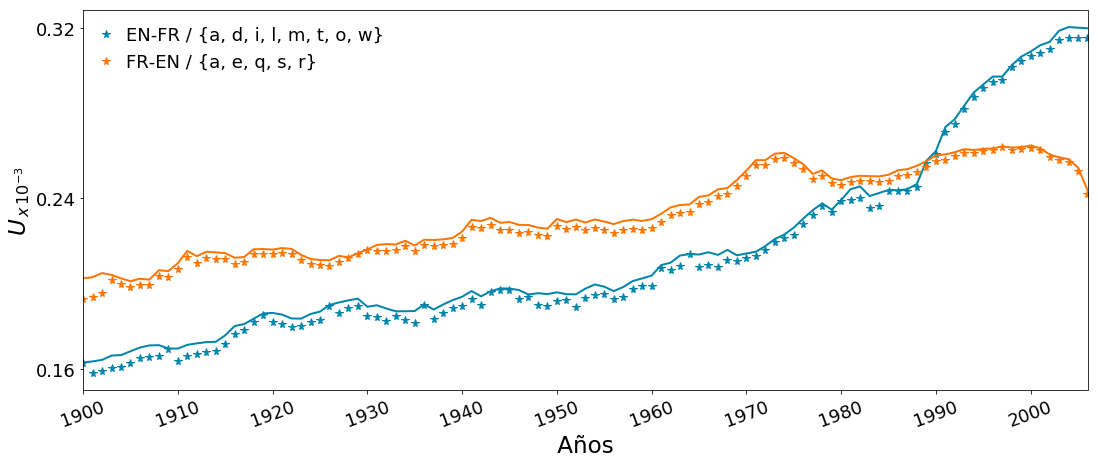
\includegraphics[scale=.375]{OM1.png}
	\label{fig.OM1}
	\caption{En ambas parejas de idiomas hay conservación del uso durante todo el siglo XX, al presentar valores iguales y  diferencia de alturas.}
\end{figure}


\begin{figure}[h!]
	\centering
	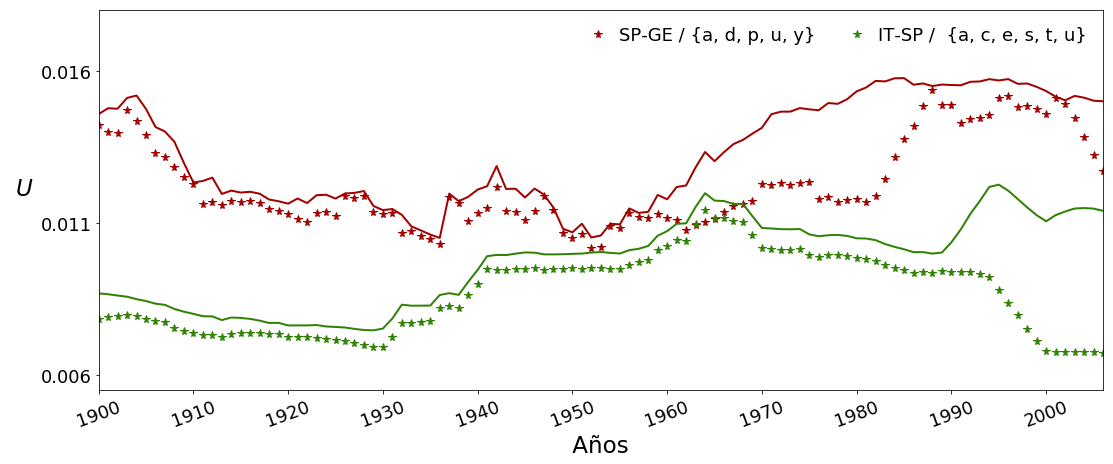
\includegraphics[scale=.375]{OM2.png}
	\label{fig.OM2}
	\caption{Sin conservación para el español-alemán entre 1960 y 1990,  debido a una alteración por periodos. Para el italiano-español el uso se conservo hasta mitad de siglo al existir una diferencia de alturas, en los últimos años se caracteriza por una alteración.}
\end{figure}

\clearpage
\begin{figure}[h!]
	\centering
	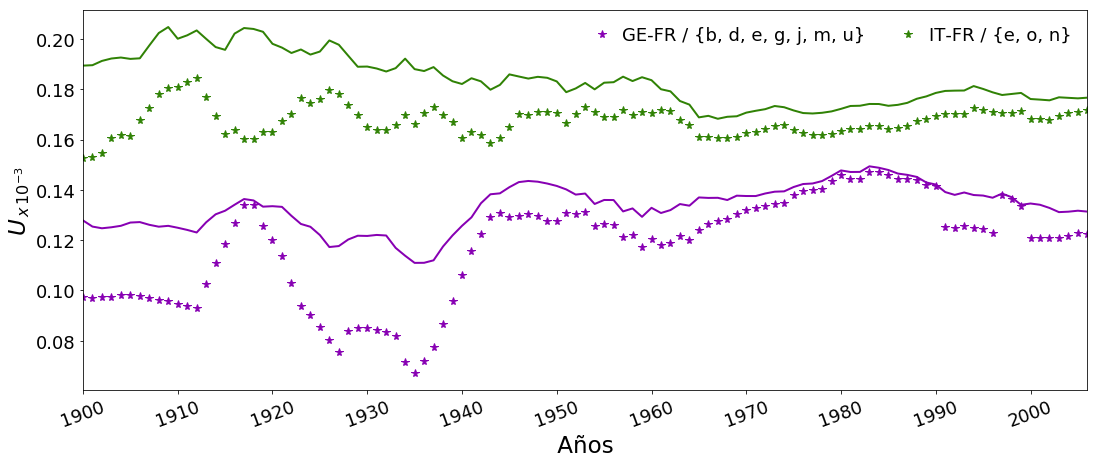
\includegraphics[scale=.375]{OM3.png}
	\label{fig.OM3}
	\caption{ En el italiano-francés se presenta conservación al  reducirse la diferencia de alturas conforme avanza el tiempo. El alemán-francés  presenta las tres características,  valores iguales  , alrededor de 1980  alteraciones entre 1920 y 1940, y deferencia de alturas  en los años restantes; la conservación dependerá del periodo  que se estudie.}
\end{figure}




El uso y la conservación no siempre serán la mismas tras una eliminación con diferentes letras, sin embargo es posible decir, de manera general si un idioma se conserva, para ello son útiles los resultados de las repeticiones. Si en cada idioma origen, se agrupan y promedian los valores del coeficiente de determinación,  se obtiene un valor promedio $\left \langle R^{2}  \right \rangle$ con el cual exponer si el origen se conserva.  Los resultados de la tabla \ref{tab.conservacion} muestran el valor de  $\left \langle R^{2} \right \rangle$ de cada origen,  así como en cuales receptores la conservación fue mayor $R^{2}_{max}$ y en cuales menor $R^{2}_{min}$.





\begin{table}[h!]
	\centering
	\begin{tabular}{cccc}
		\textbf{} & \textbf{$\left \langle R^{2} \right \rangle$} & \textbf{$R^{2}_{max}$} & \textbf{$R^{2}_{min}$} \\
		\textbf{inglés}   & 0.856 $\pm$ 0.147   &  IT 0.976 $\pm$ 0.001  & GE 0.778 $\pm$ 0.032  \\
		\textbf{francés}  & 0.839 $\pm$ 0.120   &  EN 0.951 $\pm$ 0.002  & GE 0.660 $\pm$ 0.020  \\
		\textbf{alemán}   & 0.753 $\pm$ 0.069   &  EN 0.805 $\pm$ 0.061  & SP 0.514 $\pm$ 0.332  \\
		\textbf{italiano} & 0.878 $\pm$ 0.147   &  FR 0.932 $\pm$ 0.008  & EN 0.687 $\pm$ 0.030  \\
		\textbf{español}  & 0.883 $\pm$ 0.053   &  IT 0.949 $\pm$ 0.006  & GE 0.818 $\pm$ 0.016                                                                
	\end{tabular}
	\caption{Los préstamos menos afectados por las eliminaciones son de origen español, siendo su conservación favorable en los receptores. El alemán es el que menos se conserva, afectado por ser el que menor cantidad de prestamos aporta a los demás idiomas.}
	\label{tab.conservacion}
\end{table}



\section{Comentarios del método}

El realizar diferentes elecciones para restringir a los préstamos, mostró que no importan cuales elementos conforman el corpus, la propiedad del uso es la misma. 

Individualmente los valores de uso de una única palabra pueden variar en los años de estudio y ser distintos a los de otra palabra, sin embargo al tratar a todo el conjunto, el uso se comporta de la misma  manera, sin importar los valores individuales de los elementos que lo conforman. 



